\chapter{Introduction}

\pagenumbering{arabic}


In the past few years algorithms of computer vision and especially artificial intelligence and deep neural networks brought promising results in image data processing, mostly in the tasks of object detection, semantic segmentation and classification. These advancements may have significant impact in vast number of fields, one of them being medicine. 

In medicine different types of imaging techniques are being used in order to provide both non-invasive and invasive visualizations of internal organs, tissues and other structures. Among non-invasive techniques we can count for example X-ray radiography, ultrasound imaging, magnetic resonance imaging (MRI), and computed tomography (CT). Apart from them we also mentioned invasive techniques - these are necessary when doctors need to examine a microscopic piece of tissue, e.g. potential tumour tissue or tissue that is known to be tumour - this is a discipline called histology or histopathology. Doctors can obtain the tissue either by performing biopsy or surgical resection. Biopsy is a less invasive method - it involves inserting a needle into the patients body tissue and taking out a small sample. On the other hand surgical resection is much more invasive and it involves some sort of surgical procedure during which the desired piece of tissue is removed. Depending on what doctors want to examine, these samples are then processed further. In the histopathology domain, staining of these images with chemicals is a common practice. This staining helps to create visual contrast between cells, tissues, and other objects on the image slide. Haematoxylin and eosin staining (H\&E staining) is the most widely used staining method for histopathology slides \cite{Dey2022}. Both its components are used to stain different regions of the image. Haematoxylin is responsible for colourizing cell nuclei into shades of deep blue and purple, while eosin is used for staining the extracellular matrix, cytoplasm and connective tissues in shades of pale red and pink \cite{Dey2022}. Example of this staining on a histopathology image can be seen on figure \ref{fig:h&e-image}.

\begin{figure}[h]
\begin{centering}
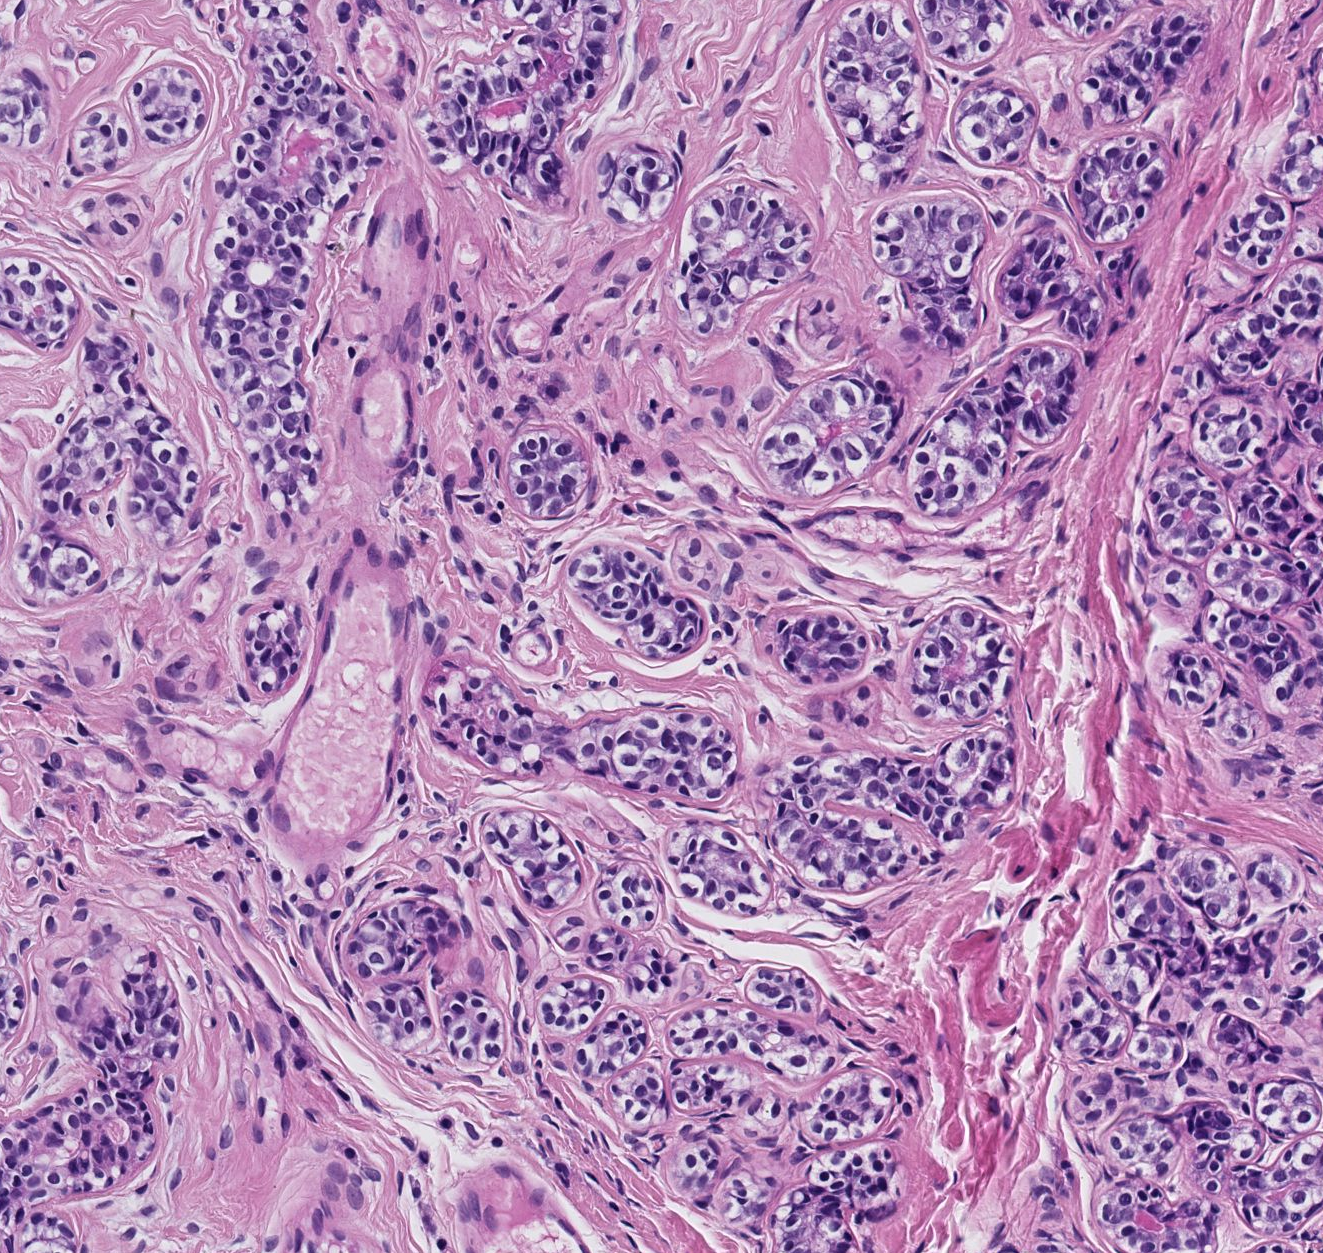
\includegraphics[width=8cm]{assets/images/histology_image_example.png}
\par\end{centering}
\caption{Example of histology image stained with haematoxylin and eosin \label{fig:h&e-image}}
\end{figure}

Slides stained by these chemicals are then examined by histopathology experts who try to identify key features which would determine a diagnosis, future treatment plan, or other subsequent steps. As a very good example of this whole process can serve a method of adjusting a treatment for patients who suffer from breast cancer.

\section{Motivation}

In recent decades breast cancer has been on of the leading causes of death among women and the second most commonly diagnosed type of cancer worldwide \cite{Bray2024, Siegel2023}. According to \cite{Bray2024} in 2022 breast cancer was attributing for approximately 2.3 million newly diagnosed patients - this represents 11.6\% of all diagnosed cancer patients in that year and 666,000 deaths, comprising 6.9\% of all cancer deaths. \cite{Siegel2023} informs that in the USA in the year of 2023 breast cancer among women accounted for more than 297,000 new cases - 31\% of all new female cancer cases and more than 43,000 deaths - 15\% of all female cancer deaths.

When dealing with breast cancer, one needs to keep in mind that there are also different subtypes of breast cancer. Firstly introduced in \cite{Perou2000}, we now know four breast cancer molecular subtypes, based on the positivity or negativity of several receptors. These receptors are Human Epidermal Growth Factor Receptor 2 (Her2) and Hormonal Receptor (HR), which is positive if either Estrogen or Progesterone receptors are positive; otherwise it is negative. These four classes along with respective receptor statuses can be seen in table \ref{tab:breast_cancer_subtypes}.

\begin{table}[H]
    \centering
    \caption{Breast Cancer Molecular Subtypes and Receptor Statuses}
    \label{tab:breast_cancer_subtypes}
    \begin{tabular}{|l|c|c|c|}
        \hline
        \textbf{Subtype Class} & \textbf{Hormone Receptor (HR)} & \textbf{Her2} \\
        \hline
        Luminal A & Positive & Negative \\
        \hline
        Luminal B & Positive & Positive \\
        \hline
        Her2-enriched & Negative & Positive \\
        \hline
        Triple Negative (TNBC) & Negative & Negative \\
        \hline
    \end{tabular}
\end{table}

From the aforementioned subtypes, the last three are the ones that currently have the worst prognosis \cite{Schalper2022, Zhang2024}. Identifying and using certain biomarkers could potentially improve the prognosis of patients with these subtypes of breast cancer. Tumour-infiltrating lymphocytes (TILs) appear as such biomarkers, especially their presence, number and spacial organization inside of the tumour and tumour-related tissue \cite{Salgado2015, Denkert2018, Amgad2019}.

However, manual identification and visual recognition of TILs from H\&E stained slides is a difficult, time-consuming, and error-prone task even when performed by experienced histopathology experts \cite{Salgado2015, Amgad2019}.

Deep learning models can be seen as a promising solution and aid for healthcare professionals in this task - by unburdening them and helping them to ease and automate the task of assessing these slides we can achieve more efficient provision of healthcare.

\section{Objectives}
Usage of a deep learning models introduces a new challenge: in order for them to lay reasonably good results, they need huge amount of high quality data \cite{Santosh2022-3}. Precise manual annotation of histology slides is not an easy nor a cheap task as we have mentioned earlier. Therefore, our aim in this work is to develop and implement a pipeline for automated detection and segmentation of tumour-infiltrating lymphocytes from breast cancer histology image slides using weak annotations, in the form of bounding boxes, of these cells. Since annotations provided are in the form of bounding boxes, our goal is two-fold:

\begin{enumerate}
    \item Develop and implement effective and precise algorithm for converting bounding box annotations into pixel mask annotations.
    \item Implement and compare various deep learning architectures, e.g. U-net and its variants or Vision Transformer and select the best one based on the evaluation metrics such as Intersection over Union (IoU) and Dice coefficient.
\end{enumerate}

In the end, we want to have a model that will be able to effectively detect and segment individual cell nuclei from weakly annotated H\&E stained histology images of breast cancer patients.

